\documentclass{article}
\usepackage{graphicx} % Required for inserting images
\usepackage[utf8]{inputenc}
\usepackage{amsmath}
\usepackage{graphicx}
\usepackage{tikz}
\usepackage{array}
\usetikzlibrary{trees}
\usepackage{amssymb}
\usepackage{amsthm}
\usepackage{multirow} 
\usepackage{dcolumn}
\usepackage{verbatim}

\newcolumntype{2}{D{.}{}{2.0}}

\title{CSC279 HW4 - Open Problem Exploration}
\author{Hanzhang Yin}
\date{Oct/18/2023}

\begin{document}

\maketitle

\noindent Picked Probelm: \textbf{Simple Linear-Time Polygon Triangulation} 
\\
\url{https://topp.openproblem.net/p10}

\subsection*{Problem Description:}
Polygon triangulation involves partitioning a simple polygon into non-overlapping triangles.
The primary challenge lies in achieving efficient algorithms that perform this triangulation in linear time, especially for large and complex polygons.

\subsubsection*{Trapezoidal Decomposition Definition: }
\textit{NOTE: we've mentioned this in the CLASS!}
\\
A key concept in Seidel's algorithm is the use of trapezoidal decomposition, where vertical lines are extended from the vertices of the polygon until they intersect other edges, forming a set of trapezoidal regions. These regions simplify the process of triangulating the polygon by breaking it into smaller, easier-to-manage pieces. Trapezoidal decomposition also plays a crucial role in other algorithms related to polygon triangulation and computational geometry.
\begin{figure*}[h]
    \centering
    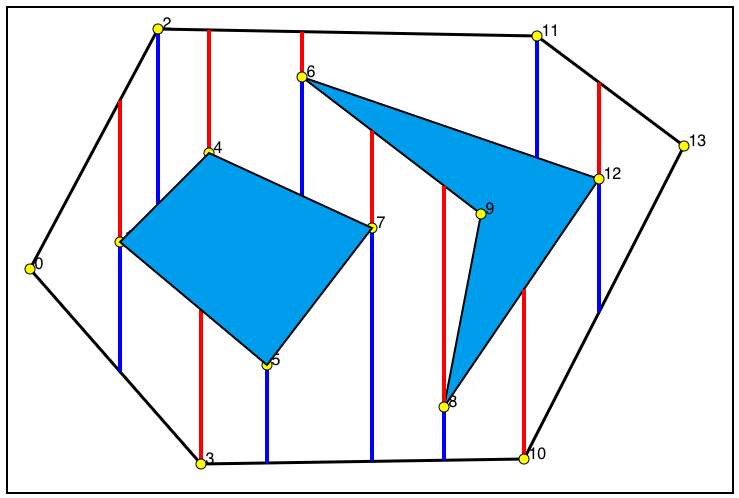
\includegraphics[width=0.7\textwidth]{TrapDecomp.png}
    \label{fig:model}
\end{figure*}

\subsubsection*{Methods to Split a Polygon into Monotone Pieces in Linear Time: }
\textit{NOTE: we've mentioned this in the CLASS as well!}
\\
To triangulate a polygon, one approach is to first decompose it into monotone pieces, which can then be efficiently triangulated. A plane sweep (or sweep line) algorithm achieves this by moving a line across the polygon and dynamically managing a list of active edges. As the \textbf{line sweeps} through, vertices are processed, and cuts divide the polygon into monotone sections.
\\
Garey, Johnson, Preparata, and Tarjan (1978) pioneered this method, showing that splitting a polygon into y-monotone pieces simplifies triangulation, allowing a linear-time algorithm. 
\\
Additionally, Delaunay triangulation methods, described by Lee and Schachter (1980), offer geometric insights, where the polygon is subdivided in a way that maximizes the minimum angle of the resulting triangles. while Delaunay triangulation is not always the optimal solution for simple polygons, their work provides useful geometric insights for approaching polygon decomposition.

\subsubsection*{Monotone Polygon Triangulation in Linear Time - A General View: }
Once a polygon has been decomposed into monotone pieces, these pieces can be triangulated efficiently. A well-known approach for this is a \textbf{stack-based algorithm}, which processes vertices of the monotone polygon in order, adding diagonals as necessary to form triangles. This algorithm runs in linear time with respect to the number of vertices, making it ideal for triangulating the monotone pieces produced by the sweep line algorithm.
\\
The stack-based approach for triangulating monotone polygons was originally introduced by Garey et al. (1978) [4], and it has become the foundation for many modern polygon triangulation algorithms. The key advantage of this approach is its simplicity: it requires only a linear scan of the vertices and a stack to store active edges.
\\
Further work by de Berg, van Kreveld, Overmars, and Schwarzkopf (2000) in Computational Geometry: Algorithms and Applications provides a detailed treatment of monotone polygon triangulation and the various approaches that can be used to achieve linear-time performance [8].

\subsection*{Approaches and Recent Developments:}
Chazelle's [1] groundbreaking 1991 algorithm was the first to achieve deterministic linear-time triangulation of a simple polygon. However, its complexity has driven researchers to seek simpler yet efficient alternatives. Recent (But not that recent) advancements include both deterministic and randomized algorithms that strive to match or approach linear-time performance with greater simplicity:
\begin{enumerate}
    \item \textbf{Randomized Algorithms: }
    One algorithm computes the trapezoidal decomposition of a simple polygon in expected linear time, enabling linear-time triangulation through known reductions. It simplifies Chazelle's method by performing random sampling [3] on subchains of the polygon rather than its edges. 
    \item \textbf{``Deterministic'' Linear-Time Algorithm: }
    Further work by Amato, Goodrich, and Ramos (2000) has explored the use of random sampling techniques to simplify the triangulation of polygons, leveraging the polygon-cutting and planar separator theorems to build a coarse triangulation in a bottom-up phase. Their method builds upon Seidel's randomized approach and shows how geometric random sampling can lead to efficient linear-time algorithms without needing complex structures [2]. 
    These advancements emphasize the practicality of randomized techniques in computational geometry, particularly for tasks such as polygon triangulation.
\end{enumerate}

\subsection*{Further Exploration: }

\subsubsection*{Seidel's algorithm Exploration: }
Seidel's algorithm offers a promising direction for further exploration, particularly due to its simplicity compared to Chazelle's deterministic method. The use of \textbf{random sampling} in Seidel’s algorithm simplifies the trapezoidal decomposition process and allows for an expected linear-time solution. Random sampling has proven to be a valuable tool in computational geometry, as demonstrated by Amato et al. (2000) [2], who further developed random-sampling techniques for geometric structures, including polygon triangulation.
\\
A possible direction for further exploration would be to investigate how the random sampling mechanism could be extended or refined to handle more complex polygons, or to simplify the overall triangulation process. Additionally, exploring hybrid approaches that combine deterministic and randomized methods might yield algorithms that are both efficient yet simple.

\subsubsection*{Connections to Delaunay Triangulation: }
While Delaunay triangulation focuses on maximizing the minimum angle of triangles, techniques from Delaunay triangulation could provide valuable insights for improving polygon triangulation algorithms. Delaunay triangulation is often used for \textbf{geometric subdivision} and has been shown to be efficient in a variety of contexts. Lee and Schachter (1980) developed algorithms for constructing Delaunay triangulations that could be adapted to polygon triangulation tasks [5].
Moreover, Dwyer's (1987) \textbf{divide-and-conquer} algorithm for Delaunay triangulation provides a fast method for constructing triangulations, and this divide-and-conquer approach could be adapted to break down the triangulation of simple polygons into smaller subproblems that can be solved in linear time [7]. Exploring how these methods can be applied to monotone polygon triangulation may yield new insights.

\subsubsection*{Exploring Ear Clipping Methods:}
Another avenue worth exploring is the ear clipping method for polygon triangulation. An ear of a polygon is a triangle formed by three consecutive vertices, where the triangle lies entirely inside the polygon and contains no other vertices. The ear clipping method works by sequentially removing ears from the polygon until only triangles remain. Meisters (1975) described how this method can be applied to polygon triangulation, and while it may not always be the most efficient method, it is simple and can be adapted for monotone polygons [6].
\\
By applying ear clipping to monotone pieces produced by a sweep line algorithm, it may be possible to achieve an efficient linear-time triangulation algorithm. Since monotone polygons have \textbf{simpler structures}, the ear clipping process can be applied without complex data structures, further simplifying the triangulation process.

\subsection*{Possible Thoughts For Approaching (Topological Approach):}
A simple linear-time algorithm for polygon triangulation can be achieved by combining the plane sweep algorithm with efficient triangulation methods for monotone polygons. First, decompose the polygon into y-monotone pieces using the plane sweep algorithm pioneered by Garey, Johnson, Preparata, and Tarjan (1978), which operates in \( O(n) \) time. Then, apply a simplified ear clipping method to each monotone piece. An "ear" is a triangle formed by three consecutive vertices that lies entirely inside the polygon without containing any other vertices. Since monotone polygons have simpler structures, ear clipping can be performed efficiently without complex data structures. This approach achieves an overall linear-time algorithm (\( O(n) + O(n) = O(2n) \)), providing a practical and efficient solution for polygon triangulation while avoiding the complexities of more intricate algorithms.
\\
Additionally, incorporating geometric insights from Delaunay triangulation, as discussed by Lee and Schachter (1980), can enhance the quality of the triangulation by maximizing the minimum angles of the triangles. Exploring randomized techniques like Seidel's algorithm or hybrid methods that combine deterministic and randomized approaches may further simplify the process without sacrificing efficiency.

\newpage

\begin{thebibliography}{9}

    \bibitem{Cha91}
    Chazelle, Bernard. 1991. “Triangulating a Simple Polygon in Linear Time.” \textit{Discrete \& Computational Geometry}, 6(3): 485-524. https://doi.org/10.1007/BF02574703.
    
    \bibitem{Amato2000}
    Amato, Nancy M., Michael T. Goodrich, and Edgar A. Ramos. 2000. “Linear-Time Triangulation of a Simple Polygon Made Easier via Randomization.” In \textit{Proceedings of the 16th Annual Symposium on Computational Geometry}, 201–212. https://doi.org/10.1145/336154.336206.
    
    \bibitem{Seidel1991}
    Seidel, Raimund. 1991. “A Simple and Fast Incremental Randomized Algorithm for Computing Trapezoidal Decompositions and for Triangulating Polygons.” \textit{Computational Geometry}, 1(1): 51–64. https://doi.org/10.1016/0925-7721(91)90012-4.
    
    \bibitem{Garey1978}
    Garey, M. R., Johnson, D. S., Preparata, F. P., & Tarjan, R. E. (1978). “Triangulating a Simple Polygon.” \textit{Information Processing Letters}, 7(4), 175-179. https://doi.org/10.1016/0020-0190(78)90076-0.
    
    \bibitem{Lee1980}
    Lee, D. T., & Schachter, B. J. (1980). “Two algorithms for constructing a Delaunay triangulation.” \textit{International Journal of Computer \& Information Sciences}, 9(3), 219-242. https://doi.org/10.1007/BF00977785.
    
    \bibitem{Meisters1975}
    Meisters, G. H. (1975). “Polygon triangulation—using ear clipping.” \textit{SIAM Journal on Applied Mathematics}, 14(2), 329-334. https://doi.org/10.1137/0114030.
    
    \bibitem{Dwyer1987}
    Dwyer, R. A. (1987). “A faster divide-and-conquer algorithm for constructing Delaunay triangulations.” \textit{Algorithmica}, 2(2), 137-151. https://doi.org/10.1007/BF01840358.
    
    \bibitem{deBerg2000}
    de Berg, M., van Kreveld, M., Overmars, M., & Schwarzkopf, O. (2000). \textit{Computational Geometry: Algorithms and Applications}. Springer. https://doi.org/10.1007/978-3-662-04245-8.
    
\end{thebibliography}

\end{document}
